\documentclass[useAMS,usenatbib]{mn2e}
\usepackage{myaasmacros}
\usepackage{graphicx}
\usepackage{ulem}
\usepackage{amsmath}
\usepackage{epstopdf}

% Some definitions of things I always use here:
\def\ltsima{$\; \buildrel < \over \sim \;$}
\def\simlt{\lower.5ex\hbox{\ltsima}}   
\def\gtsima{$\; \buildrel > \over \sim \;$}
\def\simgt{\lower.5ex\hbox{\gtsima}}
\newcommand\bcite[1]{\citeauthor{#1} \citeyear{#1}}

% Some definitions for the priors:
\def\gprior{{\tt gprior}}
\def\cprior{{\tt cprior}}
\def\bprior{{\tt bprior}}
\def\lbprior{{\tt lbprior}}

%Some definitions for rhodm etc:
\def\vztwo{\overline{v_z^2}}
\def\vztwoi{\overline{v_{z,i}^2}}
\def\rhodisc{\rho_\mathrm{disc}(z)}
\def\rhodmext{\rho_\mathrm{dm,ext}}
\def\rhodm{\rho_\mathrm{dm}}
\def\rhoeff{\rho_\mathrm{dm}^\mathrm{eff}}
\def\nuobs{\nu_\mathrm{obs}(z)}

\title[The dark matter density profile over five decades in mass]{The dark matter density profile over five decades in mass from strong lensing}

\author[Li]{Fei Li$^1$\thanks{E-mail: lif@phys.ethz.ch}, J. I. Read$^2$, J. Coles$^3$, P. Saha$^3$\\
$^1$ICFP, D\'{e}partement de Physique de l'\'{E}cole Normale Sup\'{e}rieure, 24 rue Lhomond, 75005 Paris, France\\
$^2$Department of Physics, University of Surrey, Guildford, GU2 7XH, UK\\
$^3$Institute for Theoretical Physics, University of Z\"urich, Winterthurerstrasse 190, 8057 Z\"urich, Switzerland
}

\begin{document}

\maketitle

\begin{abstract}
Abstract here. 
\end{abstract}

\begin{keywords}
\end{keywords}

\section{Introduction}\label{sec:introduction}

Large N-body cosmological simulations have been carried out with the goal of making statistical predictions on dark matter (DM) halo properties. The result suggests that these halos are self-similar, with universal density profiles \citep[see e.g.,][]{Navarro, Diemand, Hayashi, Merritt, Graham, Moore}. However, while different baryonic effects play a crucial role when it comes to the central slope of the dark matter halo density profile, most of cosmological simulations contain dark matter particles only due to numerical issues \cite[see][]{Mayer}. 

In this work, we aim to probe observationally the central density profiles of the underlying dark matter distribution of 25 lensing systems. The motivation for non-parametric mass reconstruction and the introduction to a new algorithm on non-parametric strong lensing employing the technique of pixelated lens models are given in Section \ref{parametric}. The reconstructed dark matter projected-mass maps are presented in Section \ref{mass}. In Section \ref{profile} we compare the inner density slopes of the lens sample with the result from dark matter only structure formation simulations in $\Lambda$CDM cosmology, and we discuss our results and conclude in Section \ref{sec:conclusions}.




\section{Methodology}\label{sec:method}
\subsection{Non-parametric modeling: the GLASS algorithm}\label{parametric}
For most lensed images, it is fairly easy to fit a model galaxy lens to the image positions and hence provide a map of the total sky-projected mass \citep{IF}. But such a map, although a reasonable first approximation, will be nonunique because of degeneracies. While parametric modeling is sufficient for most purposes, it is not general enough \citep{Kneib, Nata}. Mass models motivated by numerical simulations, such as the NFW profile, invoke assumptions on the nature of the particles which are simulated. Together with the increasing complexity of models - considering different matter components and a variety of physical processes - uncertainties may pile up and introduce hard to quantify departures from real matter distributions \citep{DL}. 

A way around this problem is to generate an ensemble of models, all models constrained to reproduce the observed image positions (and time delays if known) precisely. We use the GLASS code \citep{JC}, an algorithm sampling the 'model-space' with reasonable priors, with the lens model constructed as a superposition of mass pixels. Specifically, in this work we require the projected density to (i) be non-negative, (ii) be centrally concentrated, with the local density gradient pointing at most 50\degr  away from the center, and (iii) have no pixel more than twice the sum of its neighbors, the central pixel excepted. The explicit equations are given in early papers \citep{SW, Ab} for weak as well as strong lensing. The GLASS algorithm uniformly samples the model-space that satisfies all the equations and inequalities, resulting in a model-ensemble from which estimates and uncertainties can be derived.

\subsection{Disentangling matter}

As the total mass can be accessed by the GLASS program, the stellar part can be deduced using population synthesis. The stellar mass estimates are based on a comparison of surface brightness profiles with stellar mass-to-light ratios ($\Upsilon$) determined by population synthesis models for each pixel in the photometry \citep{IF,IF2}. The code used for this procedure was written by Ignacio Ferreras and relies on synthesis models and stellar spectral libraries from \citep{Bru}.

Figure \ref{f1} shows the end-product of the stellar population synthesis pipeline, a stellar surface mass map ($\Sigma _{M_s}$) in a logarithmic scale. The contours enclose pixels with stellar masses equal to or greater than the value stated in the contour labels \citep{DL}. 

\begin{figure}
\begin{center}
\hspace{-7mm}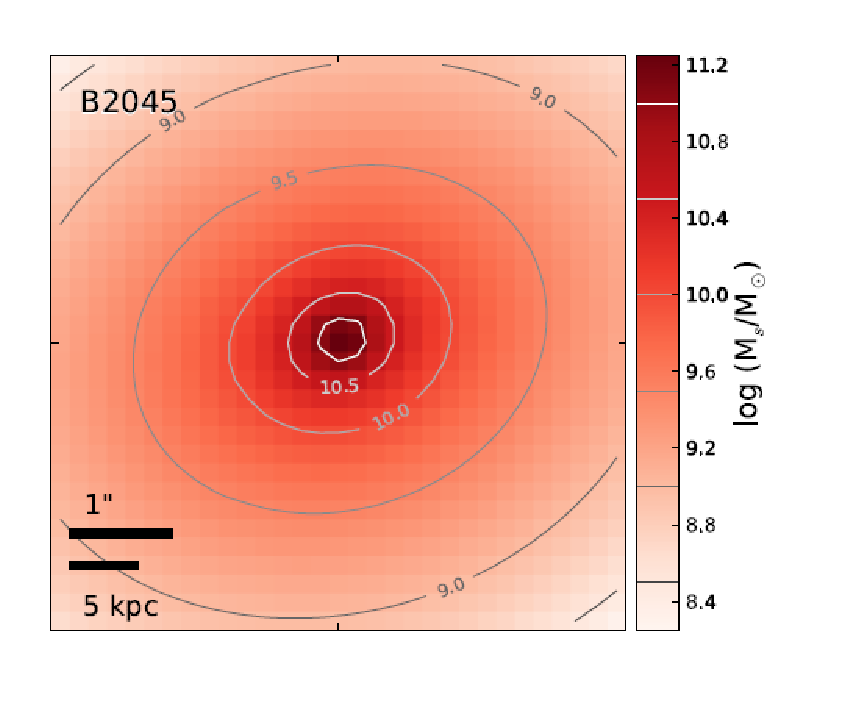
\includegraphics[height=0.29\textwidth]{f1.eps}
\caption{Projected stellar surface mass map for the lens B2045 from \citet{DL}. Note that the contours enclose pixels of same or higher stellar mass. They do not refer to the total stellar mass enclosed. The box size is 31$\times$31 pixels.}
\label{f1}
\end{center}
\end{figure}
 
\section{Result of dark matter mass reconstruction}\label{mass}

The difference between the reconstructed total mass and the stellar mass derived above is not necessarily made up of $100\%$ dark matter. Baryons which did not form stars might be stored in large more or less clumpy dust and gas reservoirs in the galaxies \citep[e.g.][]{van}. However, in our work, the dust and gas contribution to the total mass is assumed to be negligible since our sample contains only one galaxies with observable dust lanes(1608) and one late-type galaxy(2237).

A sample of 18 lensing galaxies from the CfA-Arizona Space Telescope LEns Survey (CASTLES) and cluster ACO 2667 is used for this analysis. Fig. \ref{f2} shows the mass reconstruction result from GLASS for the lens HE2149-275 as an example. 
\begin{figure*}
\begin{center}
\hspace{-7mm}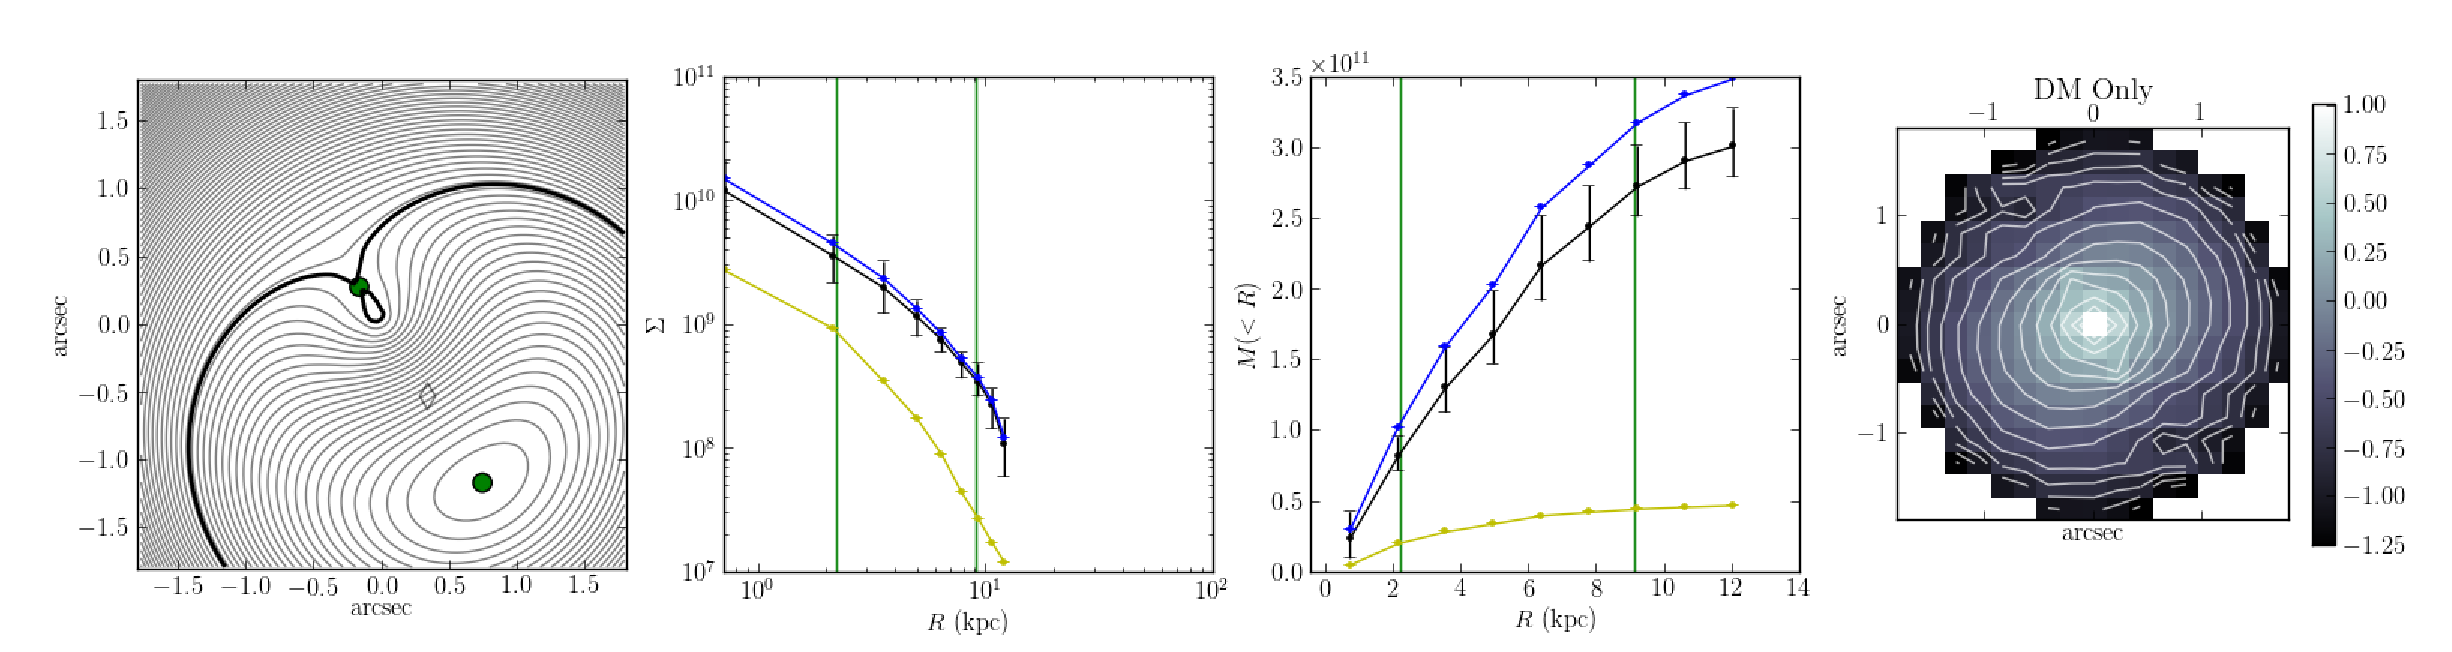
\includegraphics[height=0.27\textwidth]{f2.eps}
\caption{An ensemble of 1000 models is sampled by GLASS. Reconstructed dark matter mass map for HE2149-275 is shown in the last panel in terms of the critical mass. The first panel is the reconstructed arrival time surface, the projected density profile obtained by circularly averaging the projected-mass map is shown in the second panel (blue for total mass, black for dark matter mass and yellow for stellar mass), the enclosed projected mass is shown in the third panel.}
\label{f2}
\end{center}
\end{figure*}


\section{Dark matter density profiles} \label{profile}

Starting with the model ensemble, we circularly average each projected-mass map to obtain a $\Sigma(R)$ as shown in the second panel of Fig. \ref{f2}. We then use the ensemble of $\Sigma(R)$ to fit for the parameters in the projected generalized NFW profile parametrized with the inner logarithmic slope $\alpha$, scale length $a$ and total mass $M$
using a MCMC program. Appendix...

$M_{200}$. define $\beta$. Fig. \ref{range}. The dark matter central logarithmic density slopes from the MCMC program are shown in Fig. \ref{alpha} as a function of $M_{200}$. 

\begin{figure*}
\begin{center}
\hspace{-7mm}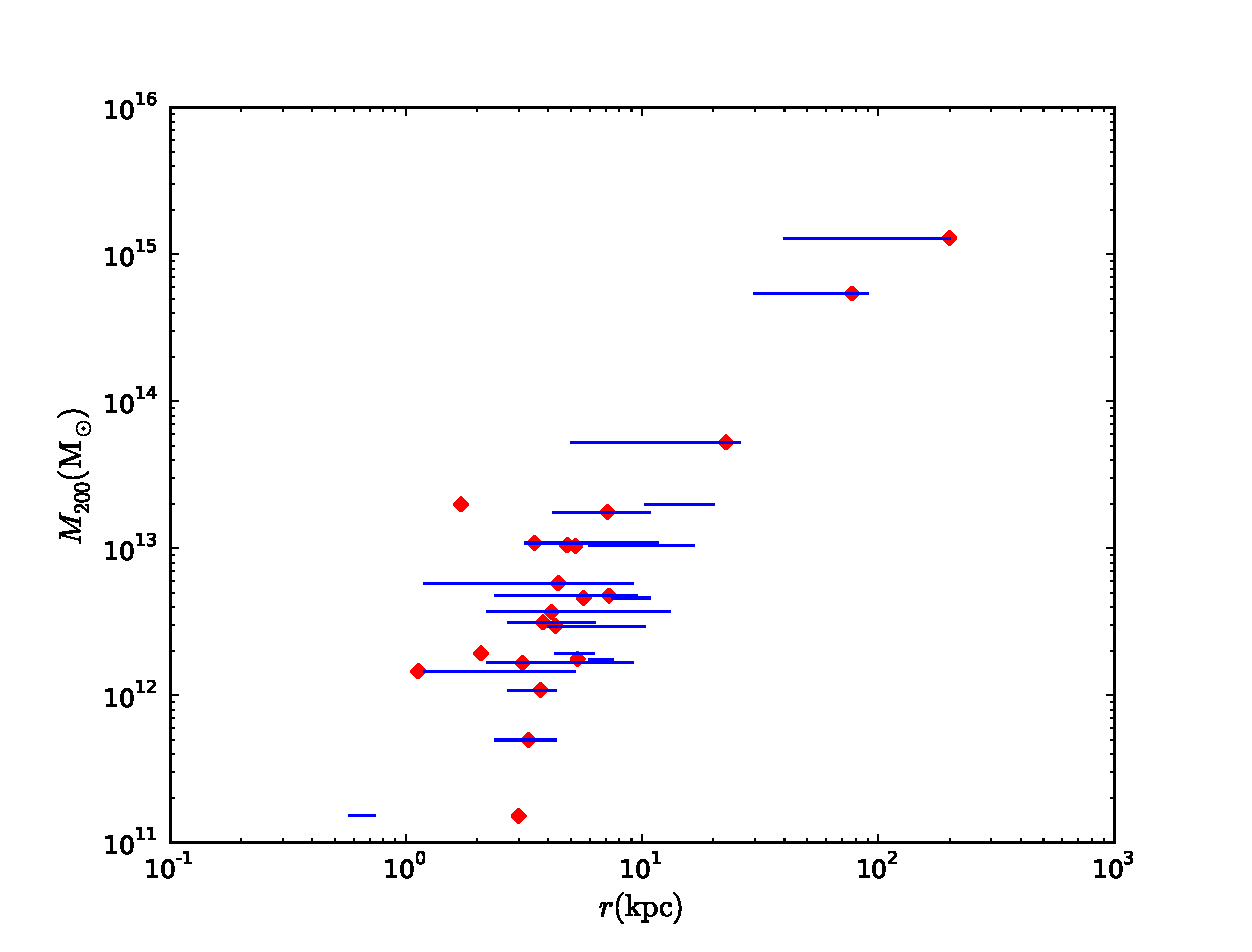
\includegraphics[height=0.44\textwidth]{range.eps}
\caption{The solid lines show the regions between the innermost image and outermost image of the lensing systems, the half light radii are marked by the red diamonds.}
\label{range}
\end{center}
\end{figure*}

\begin{figure*}
\begin{center}
\hspace{-0mm}\includegraphics[height=0.30\textwidth]{Figures/alpha04.eps}
\hspace{-0mm}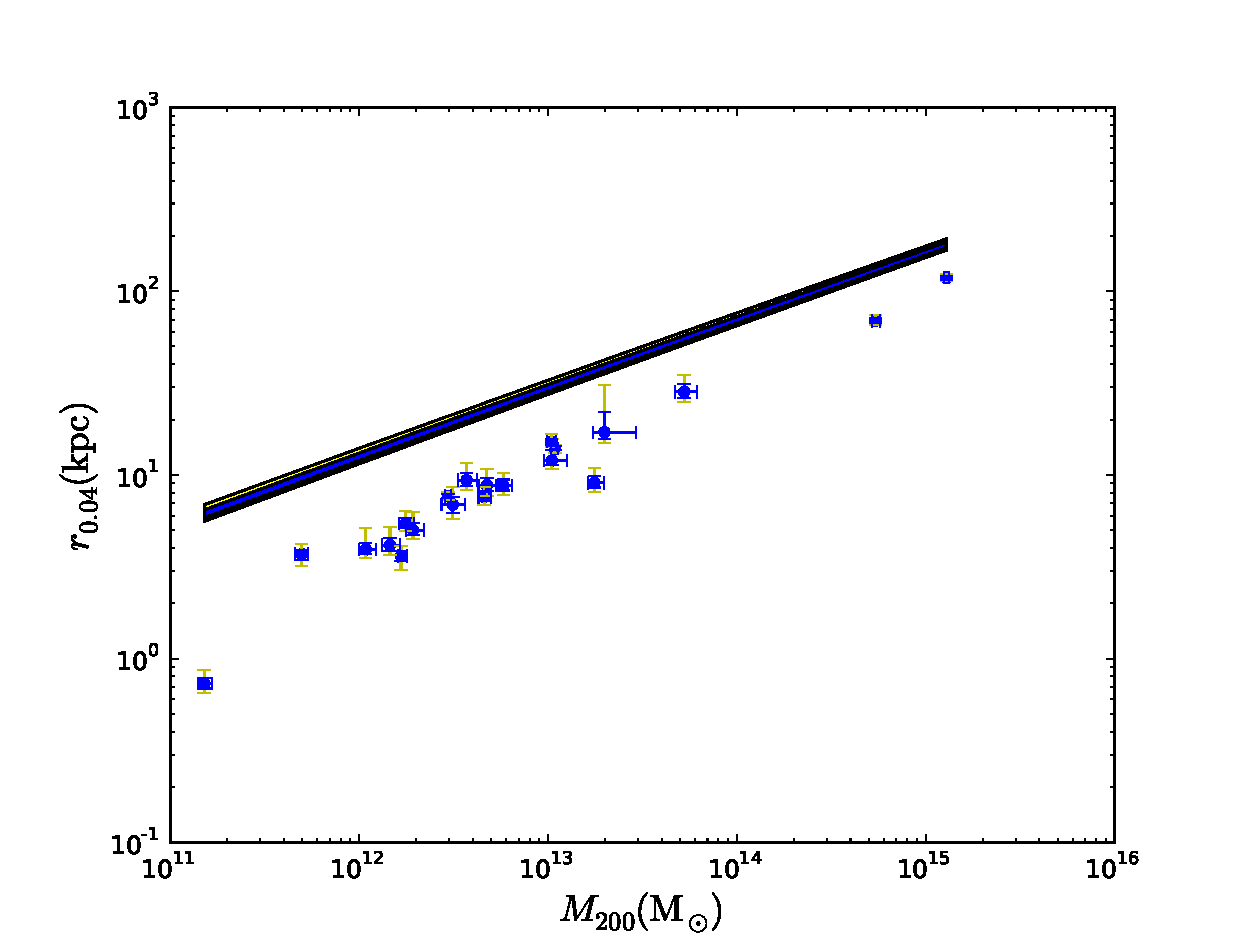
\includegraphics[height=0.30\textwidth]{Figures/r04.eps}\\
\hspace{-0mm}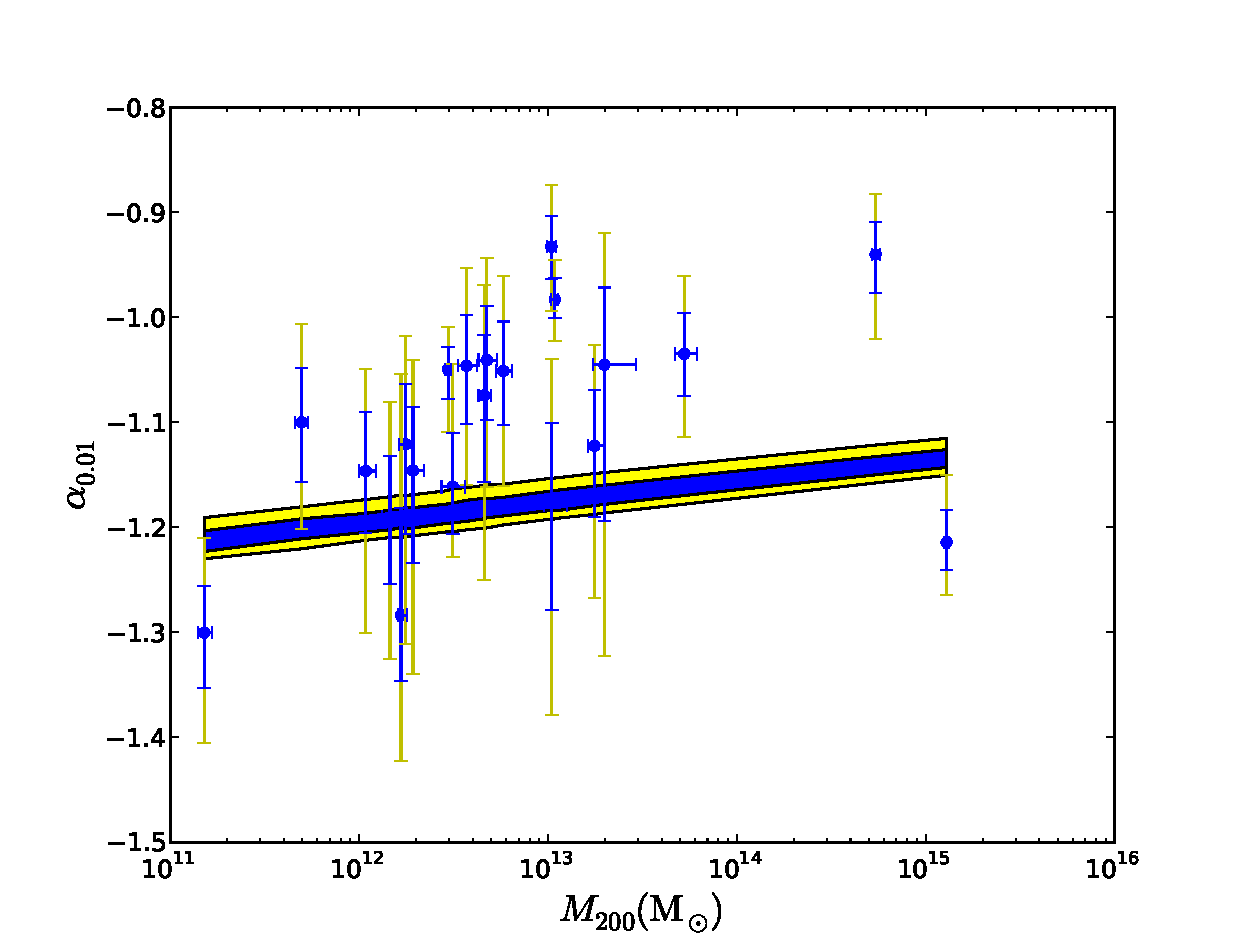
\includegraphics[height=0.30\textwidth]{Figures/alpha01.eps}
\hspace{-0mm}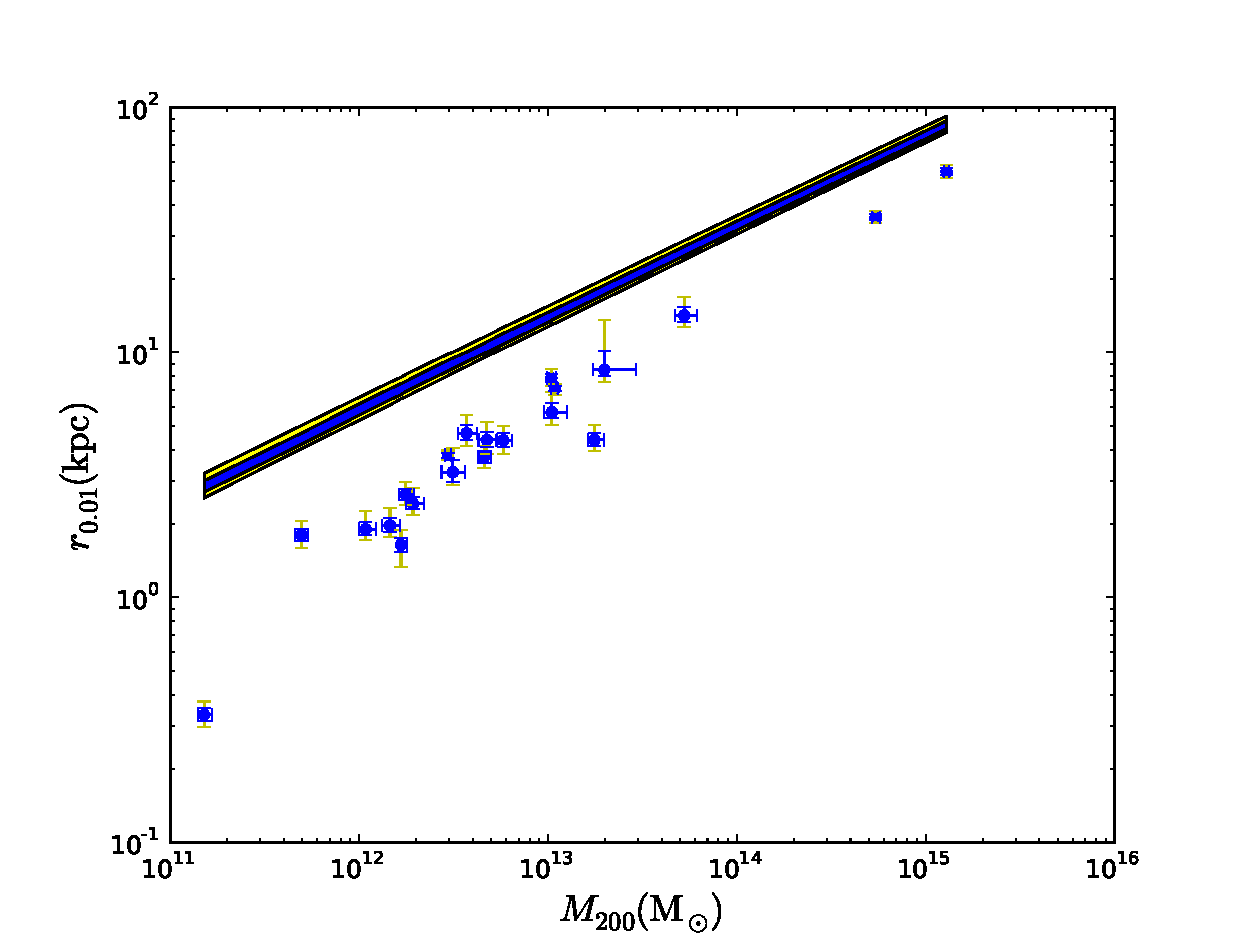
\includegraphics[height=0.30\textwidth]{Figures/r01.eps}\\
\hspace{-0mm}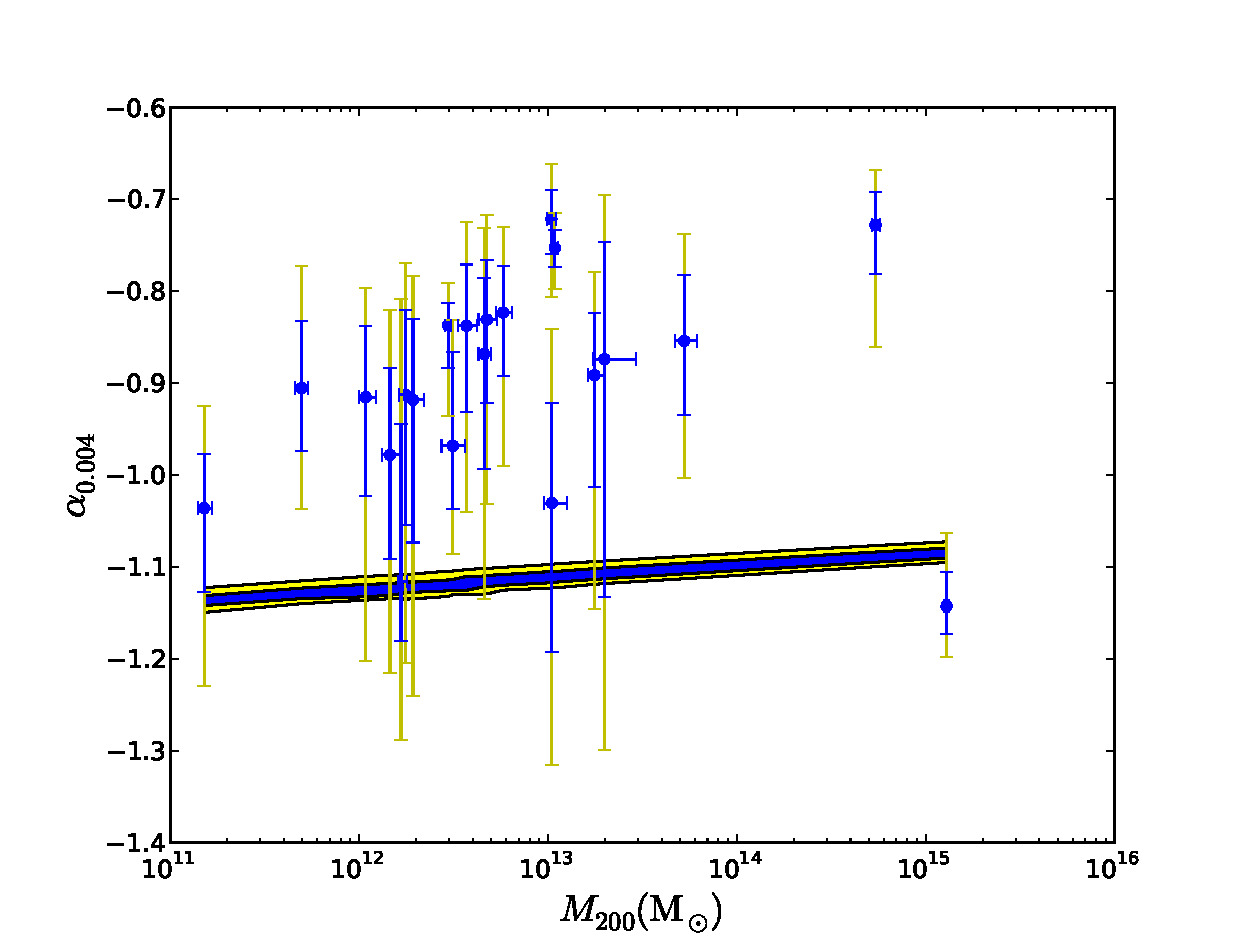
\includegraphics[height=0.30\textwidth]{Figures/alpha004.eps}
\hspace{-0mm}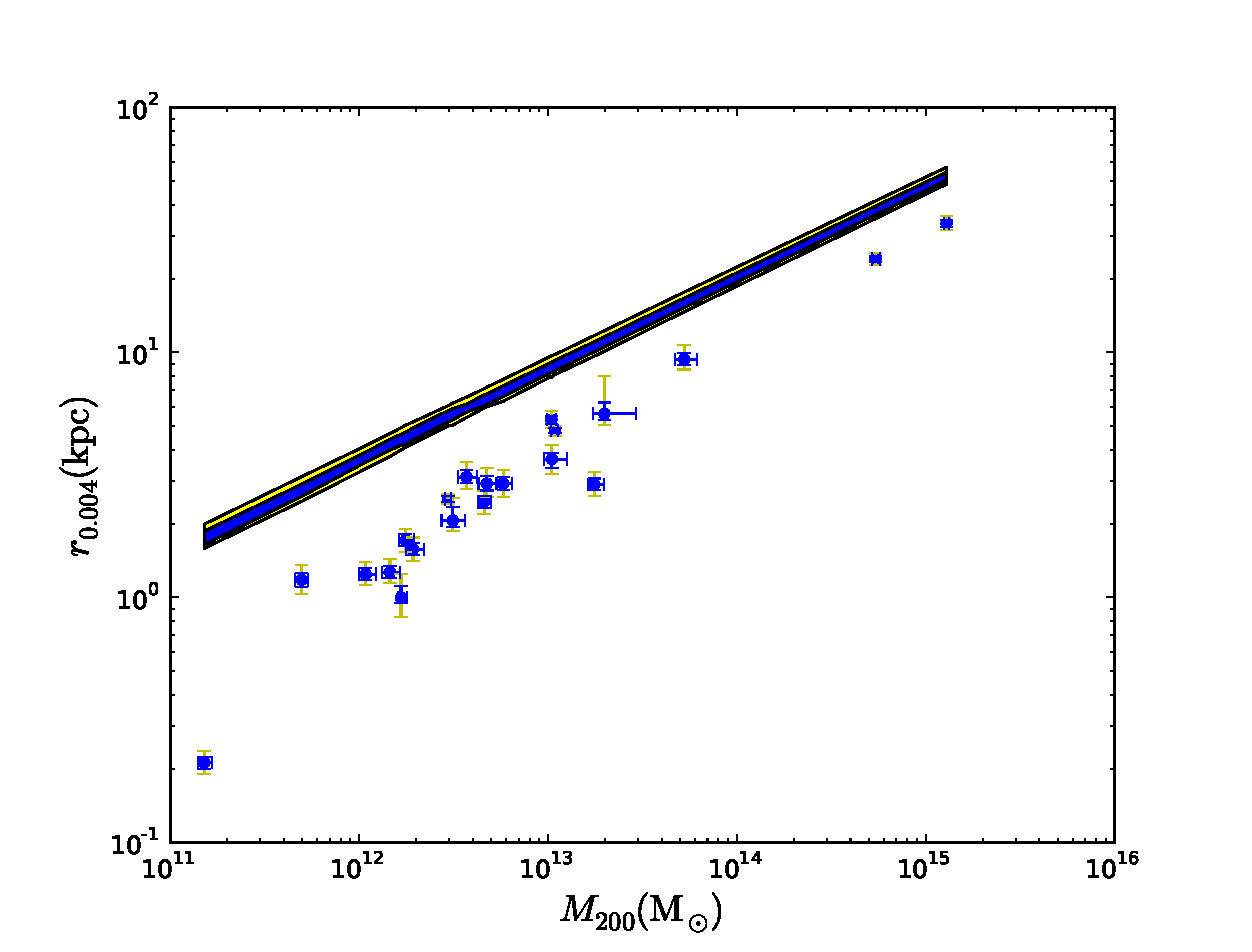
\includegraphics[height=0.30\textwidth]{Figures/r004.eps}\\
\caption{.}
%The dark matter central logarithmic density slope as a function of enclosed projected mass. 1-$\sigma$ errors are marked. A galaxy cluster is included in the right panel. The prediction \citep{DM} from dark matter only structure formation simulations (assuming non-relativistic cold dark matter) is marked by the horizontal red line; the dotted lines show the 1-$\sigma$ errors.
\label{alpha}
\end{center}
\end{figure*}

\section{Conclusions}\label{sec:conclusions}
Conclusions. 

\section{Acknowledgements}
JIR would like to acknowledge support from SNF grant PP00P2\_128540/1.


\bibliographystyle{mn2e}
\bibliography{../../BibTeX/refs}

\end{document}
